% Vorbereitung: Vorbereitungsaufgaben bearbeiten
% Versuchsaufbau: Verwendete Apparatur, Beschreibung Funktionsweise/Nutzen mit Skizze/Foto
\section{Durchführung}
\label{sec:durchführung}

Der Versuchsaufbau besteht aus einer radioaktiven Thallium-Quelle, dem Geiger-Müller Zählrohr und der daran angeschlossenen
Nachweiselektronik. Probe und Zählrohr, sowie ein Amperemeter befinden sich innerhalb einer Aluminiumabschirmung. Die zugehörige Spannungsquelle,
Verstärker und Zähler, sowie ein digitales Oszilloskop sind außerhalb angeschlossen. Diese Anordnung ist in Abbildung \ref{fig:aufbau} dargestellt.
Zunächst wird die Zählzeit auf $\increment t = \qty{120}{\second}$ festgelegt.

\begin{figure}[H]
	\centering
	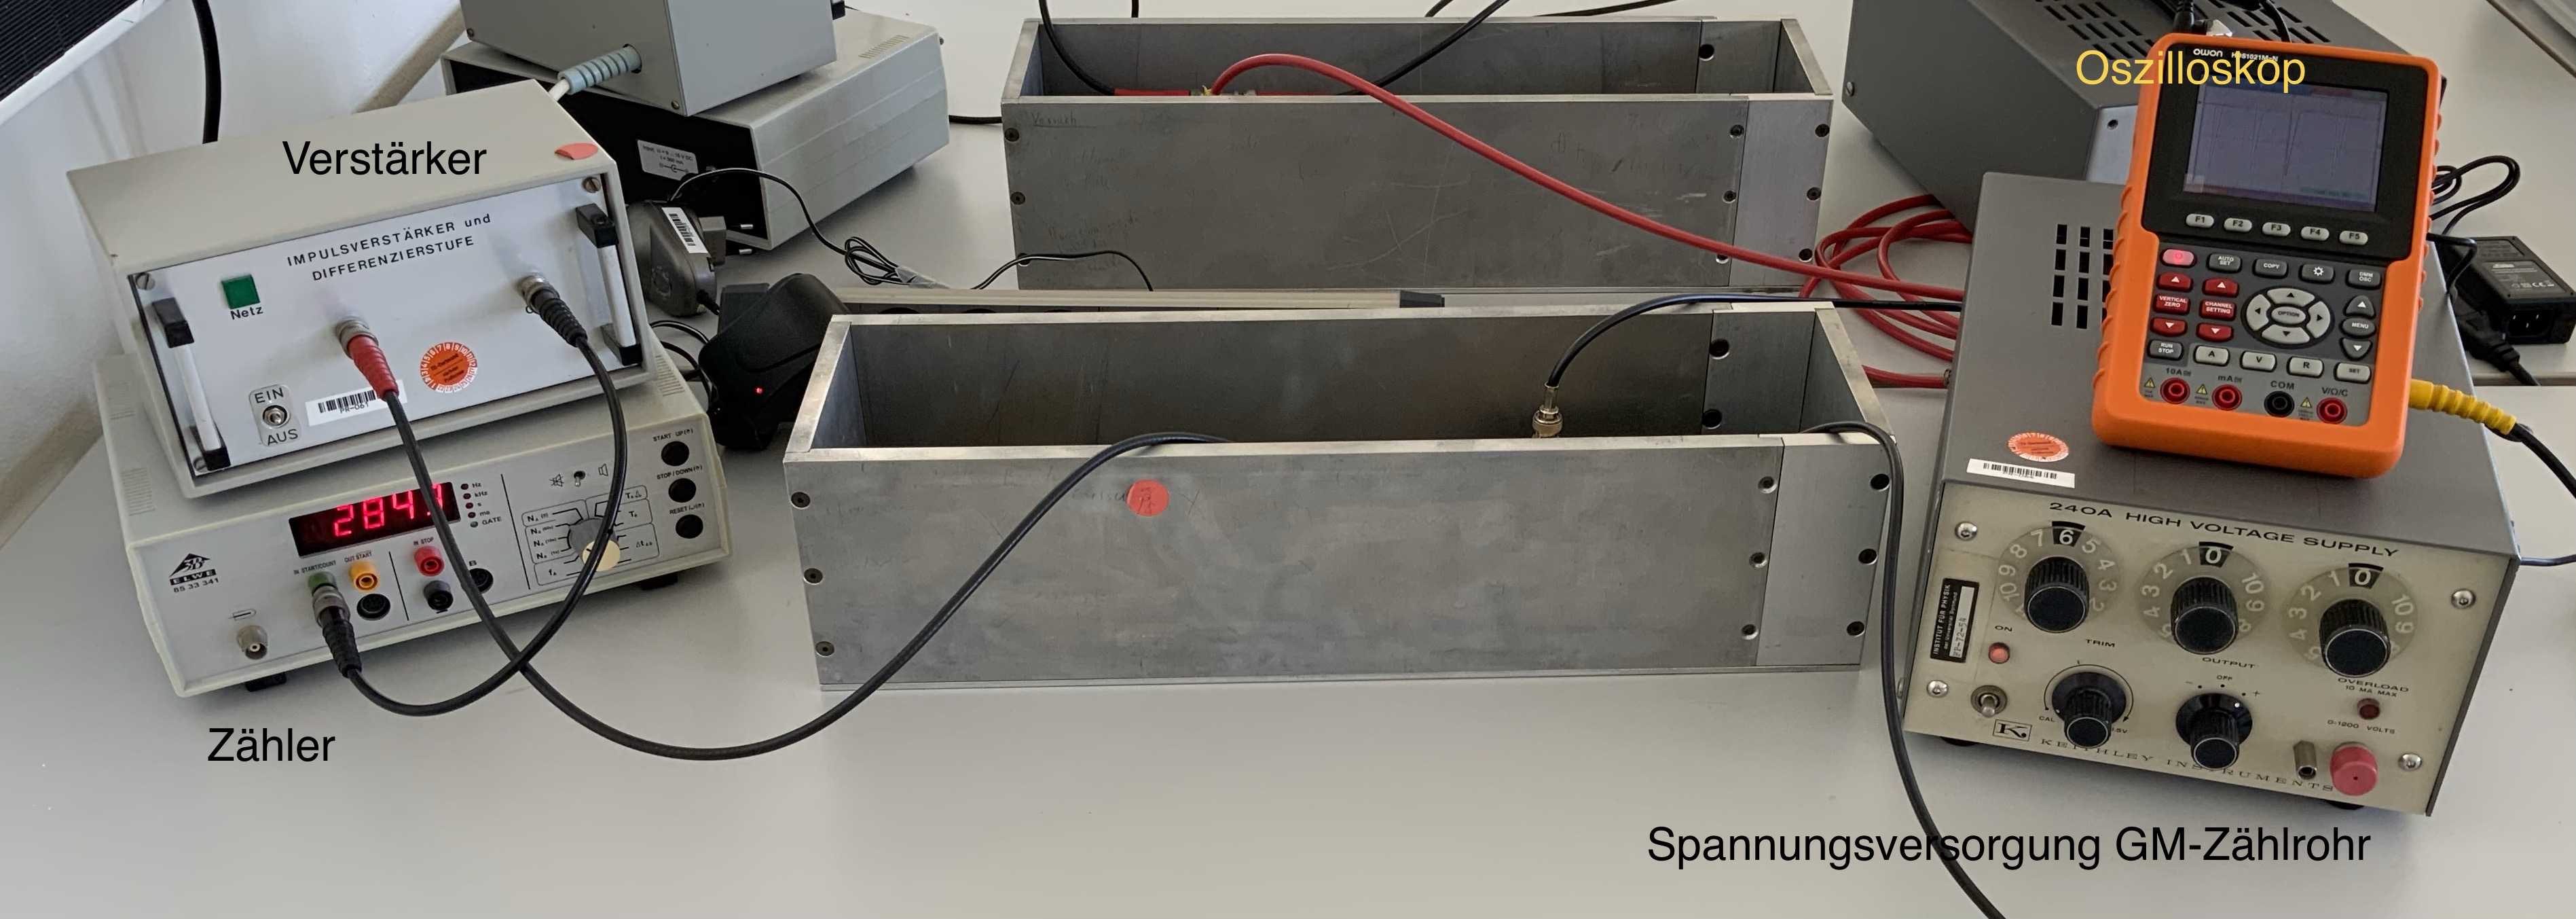
\includegraphics[width=0.9\linewidth]{content/grafik/aufbau.jpg}
	\caption{Aufbau der verwendeten Messanordnung.}
	\label{fig:aufbau}
\end{figure}

Zur Aufnahme der Kennlinie um den Geiger-Müller Bereich wird nun die Speisespannung ab $\qty{330}{\volt}$ in Schritten von $\qty{20}{\volt}$
bis $\qty{750}{\volt}$ hochgeregelt, zu jeder Spannungsstufe wird die Zählrate über das volle Messintervall nachgehalten. Hier ist zu beachten,
dass der Abstand von Quelle zu Detektor so eingestellt ist, dass der Zähler bei einer Spannung von $\qty{550}{\volt}$ weniger als $\num{2000}$
Impulse pro Sekunde registriert. Auf diese Weise lässt sich der Einfluss der Totzeit $\tau$ minimieren. Gleichzeitig wird die zur
Betriebsspannung gehörige Stromstärke notiert. Anhand dieser kann anschließend die Anzahl der Ladungsträger ermittelt werden.

Mithilfe der so gewonnenen Daten wird der Arbeitspunkt in das erste Drittel des Geiger-Müller Plateaus gelegt, die Spannung wird darauf
eingestellt. Der Abstand sollte so reduziert werden, dass die Zählrate jetzt über $\num{2000}$ Ereignissen pro Sekunde liegt. In dieser
Konfiguration wird nun für die erste Thallium-Quelle, die Quelle zusammen mit einer weiteren Probe, und schließlich die zweite Thallium-Probe
alleine je die Zählrate aufgenommen, um daraus die Totzeit $\tau$ zu berechnen.

Zuletzt wird die Detektorspannung kurzzeitig in den Bereich der Townsendentladung erhöht, um anhand des Oszilloskopschirms Auslösezeit $\tau$
und Erholungszeit $\Tau$ abzulesen.

\subsection{Vorbereitung}

Das verwendetet Isotop $\ce{^{204}_{81}Tl}$ hat eine Halbwertszeit von $3$ Jahren und $284$ Tagen und besitzt folgende
Zerfallskanäle \cite{204_tl}: Mit einer Wahrscheinlichkeit von $\qty{97.08}{\percent}$ erfährt dieses Betazerfall $(\beta^-)$ zu
$\ce{^{204}_{82}Pb}$ mit einer Halbwertszeit über $\qty{1.4e17}{Jahren}$. In den weiteren $\qty{2.92}{\percent}$ der Zerfälle
tritt Elektroneneinfang $(\varepsilon)$ auf, bei dem Produkt $\ce{^{204}_{80}Hg}$ handelt es sich dann um ein stabiles Isotop.

Um eine statistische Messunsicherheit von $\sigma_\text{rel} = \qty{1}{\percent}$ zu erhalten, muss nach Ausdruck~\eqref{eqn:relativ}
eine Zählrate von $N = \num{10000}$ erreicht werden.
